\chapter{对 ZUC 算法的分析方案}
\label{chap:attack}

\section{差分功耗分析的一般步骤}
\label{sec:dpa}
功耗分析通常包含简单功耗分析(Simple Power Analysis)和差分功耗分析(Differential Power Analysis)。

简单功耗分析通常只需要少量的功耗曲线,就能揭示密码设备中的有用信息。简单功耗分析通常适用于功耗曲线特征较为明显的密码设备,比如出现明显的波峰和波谷,以及呈现出多个周期性的重复段落。如果攻击者对密码设备中运行的程序有一定的预备知识,那么就能推测出功耗曲线的不同段落在执行何种操作,就有可能进一步掌握设备的更多信息。

差分功耗分析则需要大量的功耗迹。大量功耗数据带来的好处就是更强大的分析和攻击能力,也不需要对设备的构造和执行的程序有详细的了解,一般情况下,只要掌握设备运行的算法流程就足够实施分析和攻击了。

因此,我们的关注重点就放在差分功耗分析上。

\vspace*{0.5\baselineskip}

下面我们来介绍一下差分功耗分析的一般流程:\cite{paa_cn}

\begin{enumerate}
\item \textbf{选取合适的算法中间值位置:}一个好的中间值,应该尽可能地区错误的猜测和正确的猜测。因此,在密码算法中,通常选择非线性函数的输出作为差分功耗分析的中间值。由于在运行算法和采集功耗时,攻击者往往只能获得明文或者密文,因此通常只能对算法的第一轮加密或者最后一轮加密进行攻击。因此,选取的中间值最好能够出现在第一轮或者的最后一轮。选取不同的中间值,会对攻击效果产生很大的影响,因此需要根据不同的算法和具体的实验条件,选取最合适的算法中间值。
\item \textbf{采集设备运行时的实际功耗曲线:}这一部分没有什么技术难度,不过值得一提的是,如果合理地选择功耗曲线采集和结束的位置,就能得到对齐较好的曲线,方便后续的分析和处理。采集环境也要尽可能地排除外界因素的干扰,以提高功耗曲线同数据和操作的相关性,增大信号的信噪比。更多具体的细节已经在上一小节阐述了。
\item \textbf{根据算法计算理论中间值:}对某个具体的密码算法而言,密钥通常是最重要也是最机密的信息,攻击者唯一无法知晓的也是这一部分。对全部位数的密钥进行穷举猜测是不可能做到的,因此攻击者常常需要在选择合适的中间值的前提下,尽可能地降低中间值和全部密钥之间的相关性。或者说,攻击者应该尽可能选取只依赖少部分密钥的中间值,这样就能大大减少猜测的可能情况,提高攻击的效率。由于密码算法通常是公开透明的,因此已知明文和猜测密钥的情况下,是可以计算出适合的理论中间值的。
\item \textbf{使用合适的功耗模型将理论中间值转换为假设功耗值:}算法的中间值通常是某个字节或者比特,和算法有关。由于中间值的值域很大,因此对所有可能的中间值建立一个具体的模型是不现实的。所以有必要采用合适的功耗模型,缩小猜测空间,将中间值转换成假设功耗值。常用的功耗模型包括汉明重量模型、汉明距离模型以及零值模型。功耗模型之间各有利弊,需要根据实际的实验情况和攻击效果选取最合适的模型。
\item \textbf{分析假设功耗值和实际功耗曲线,挖掘所需的信息:}这部分通常涉及到一定的统计学知识,需要攻击者具备较好的数学基础。在分析曲线的特征之前,通常还要对功耗曲线进行预处理,比如对齐和滤波,减少噪声,提高信噪比,从而能够更好地利用功耗曲线中的有效信息。此外,高效地处理大量的数据也是一个需要仔细考量的问题,差分功耗分析往往会采集成千上万甚至是百万条曲线,如何编写性能优异的算法,或者是并行化处理,都会很大程度上影响分析的速度和效果。除了常用的相关系数攻击之外,模板攻击也很有效。攻击者应该尽可能地设计好的算法,从而减少所需的功耗曲线条数,这样就能大大减少攻击的时间和成本。
\end{enumerate}

\vspace*{0.5\baselineskip}

图 \ref{fig:dpa} 展示了差分功耗分析攻击的第 3 -- 5 步。

\begin{figure}[htbp]

    \centering
    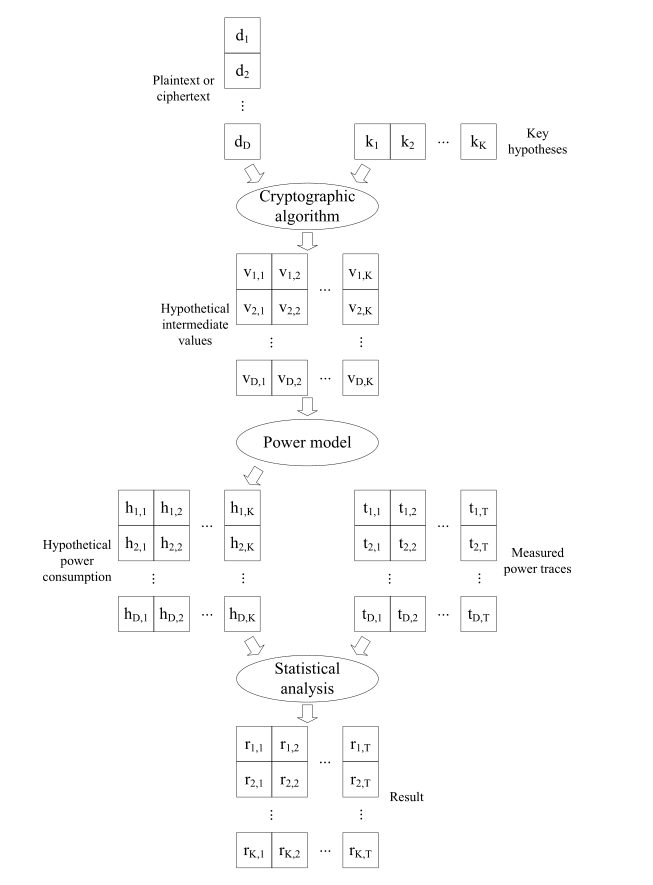
\includegraphics[height=.6\textheight]{../images/dpa.png}
    \caption{差分功耗分析的典型流程\cite{paa_en}}
    \label{fig:dpa}
\end{figure}

\section{寻找 ZUC 算法的中间值}

在进行软件分析之前,我们首先要在硬件上实现 ZUC 算法电路,并采集其运行时的功耗。这部分相对简单,我们已经在 \ref{sec:hardware} 节中实现了硬件电路,而采集功耗的过程也很容易,因此这里不再赘述。

在 ZUC 算法中,唯一未知的信息就是初始的种子密钥,其他的常量和明文都是已知的。因此我们的攻击目的就是得到密钥的信息,也就是种子密钥的各个字节。

差分功耗攻击最核心的思想是,假设功耗值和实际功耗值之间是有关联的。而要想假设功耗值尽可能贴合实际功耗值,就需要选择合适的中间值。

一般而言,中间值通常选择算法中非线性变换的部分,因为如果输入稍有不同,非线性变换的输出就会出现较大的差异,从而正确的输入和错误的输入产生的差异将比线性变换更加明显,就可以有效地区分出正确的输入和错误的输入。

因此,我们第一步想到的是,把目光放在 ZUC 算法的非线性函数模块,看看能否从这个模块的附近找到合适的中间值。

由于 ZUC 算法是分成三层的,第三层的非线性函数模块的输入,取决于第一层的线性反馈移位寄存器模块和第二层的比特重组模块的输出,而上面两层都对算法中的变量作了很多操作和运算,比如移位、剪切、粘贴、比特加、比特异或、素域模加,这就导致不同密钥字节彼此间的关联度很高。

密钥字节关联度很高的后果就是,我们很难对单个密钥字节进行猜测(只需要穷举 $2^8$ 种情况),这就导致我们必须穷举更多的情况(N 个密钥字节就对应 $2^{8 \times N}$ 中情况),一旦关联的密钥字节数较多,就几乎不可能对其穷举。

所以我们的首要任务,就是找到算法中尽可能独立的密钥字节。换句话说,如果在某个时刻,非线性函数模块的输出只和单个密钥字节相关,那么这个密钥字节就具有极强的独立性,我们也只需要穷举 $2^8$ 种情况就能攻出这个密钥字节。

我们需要对算法进行自顶向下地剖析,观察不同阶段哪些密钥字节参与了什么运算。

我们从图 \ref{fig:zuc_algo} 中截取一部分,得到图 \ref{fig:zuc_lfsr_br},该图展示了线性反馈移位寄存器模块的输出、比特重组模块的全部以及非线性函数模块的输入。

\begin{figure}[htbp]
    \centering
    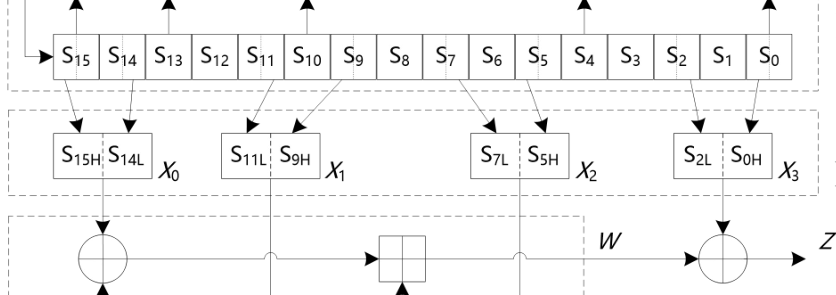
\includegraphics[width=0.8\textwidth]{../images/zuc_lfsr_br.png}
    \caption{线性反馈移位寄存器模块的输出、比特重组模块的全部以及非线性函数模块的输入}
    \label{fig:zuc_lfsr_br}
\end{figure}

从图中可以看出,并不是任何时刻所有种子密钥字节都参与算法,以初始化阶段为例,每运行一次 {\cnsls zucInit} 函数,线性反馈移位寄存器输出到下一层只同 8 个寄存器字节变量相关。影响线性反馈移位寄存器输出的便是比特重组的输入,见代码 \ref{lst:bitreorganization},我们这里将其再次写出来,方便参阅:

\begin{lstlisting}[style=myPython]
def bitReorganization():
    global x, s
    x[0] = s[15][0:16] + s[14][-16:]
    x[1] = s[11][-16:] + s[9][0:16]
    x[2] = s[7][-16:] + s[5][0:16]
    x[3] = s[2][-16:] + s[0][0:16]
\end{lstlisting}

那么这里 {\cnsls s} 又和什么有关呢?在变量初始化的代码 \ref{lst:varsinit} 中,我们可以找到如下语句:

\begin{lstlisting}[style=myPython]
...

def varsInit():
    ...
    for i in range(0, 16):
        s[i] = k[i] + d[i] + v[i]
    ...
\end{lstlisting}

也就是说,在 ZUC 算法中,线性反馈移位寄存器的每个 31 比特单元变量 {\cnsls s[i]} 是由种子密钥字节 {\cnsls k[i]}、给定的字符串常量单元 {\cnsls d[i]} 以及初始向量(输入的明文)字节 {\cnsls v[i]} 连接而成的。(可以参考表 \ref{table:symbol} 中各符号的说明。)

那么我们就可以对输入比特重组模块的 8 个字节进行拆解,找到和其相关的密钥字节:

\begin{lstlisting}[style=myPython]
    x[0] = s[15][0:16] + s[14][-16:]
         = (k[15][:] + d[15][0:8]) + (d[14][-8:] + v[14][:])

    x[1] = s[11][-16:] + s[9][0:16]
         = (d[11][-8:] + v[11][:]) + (k[9][:] + d[9][0:8])

    x[2] = s[7][-16:] + s[5][0:16]
         = (d[7][-8:] + v[7][:]) + (k[5][:] + d[5][0:8])

    x[3] = s[2][-16:] + s[0][0:16]
         = (d[2][-8:] + v[2][:]) + (k[0][:] + d[0][0:8])
\end{lstlisting}

这里提一句,在 Python 中,{\cnsls s[15][0:16]} 表示 {\cnsls s[15]} 的前 16 比特,也就是第 0 到 15 比特,而不是第 0 到 16 比特,相当于索引的区间是左闭右开。{\cnsls s[14][-16:]} 则表示 {\cnsls s[14]} 的末 16 比特,{\cnsls k[15][:]} 表示 {\cnsls k[15]} 的全部比特(8 位)。

从拆解结果可以看到,相关的密钥字节有且仅有:{\cnsls k[15], k[9], k[5], k[0]}。

那么,在非线性函数模块中,是不是这 4 个又都参与运算了呢?并不是。

我们再截取图 \ref{fig:zuc_algo} 的另外一部分,得到图 \ref{fig:zuc_br_f},稍作观察。

\begin{figure}[htbp]
    \centering
    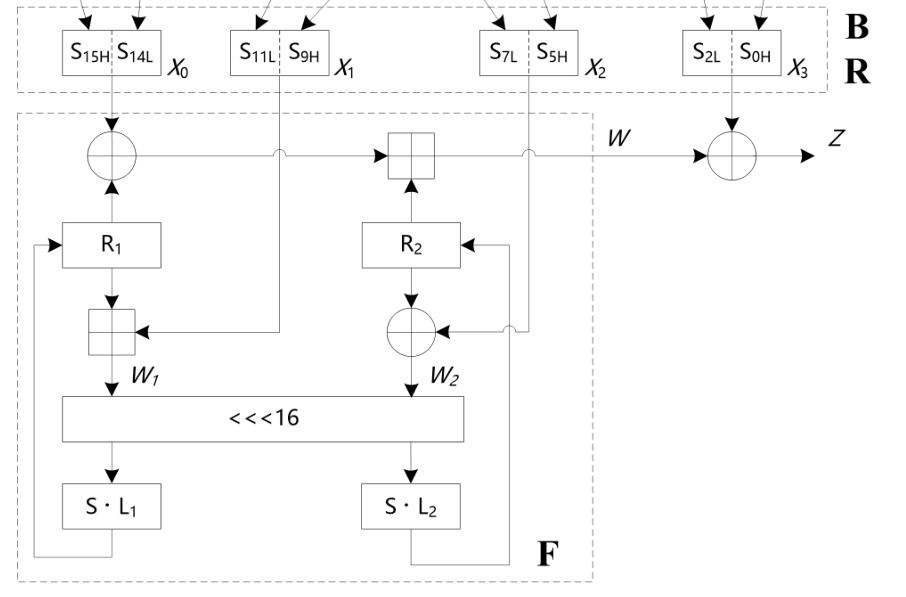
\includegraphics[width=0.8\textwidth]{../images/zuc_br_f.png}
    \caption{比特重组模块和非线性函数模块}
    \label{fig:zuc_br_f}
\end{figure}

从图中的数据流向可以看出,{\cnsls x[0]} 和 {\cnsls x[3]} 并没有参与非线性函数模块的内部操作,而只是和记忆单元 {\cnsls r1} 和 {\cnsls r2} 作了简单的运算,用于输出密钥流。

因此,真正参与非线性函数模块的内部操作的,只有 {\cnsls x[1]} 和 {\cnsls x[2]},与之相关的密钥字节便是 {\cnsls k[9]} 和 {\cnsls k[5]}。

下面我们再来看一下 {\cnsls k[9]} 和 {\cnsls k[5]} 又是如何参与非线性函数中的运算的。

这里我们将非线性函数模块的代码 \ref{lst:nonlinearfunction} 重写一遍,方便查看:

\begin{lstlisting}[style=myPython]
def nonLinearFunction():
    global w, x, r1, r2
    w = binaryAdd(binaryXor(x[0], r1), r2)
    w1 = binaryAdd(r1, x[1]) `\label{line:w1}`
    w2 = binaryXor(r2, x[2]) `\label{line:w2}`
    r1 = sboxOfZuc(linearTransform(w1[-16:]+w2[0:16], 1)) `\label{line:r1}`
    r2 = sboxOfZuc(linearTransform(w2[-16:]+w1[0:16], 2)) `\label{line:r2}`
\end{lstlisting}

从第 \ref{line:r1} -- \ref{line:r2} 行可以看出,{\cnsls r1} 和 {\cnsls r1} 的值同 {\cnsls w1} 和 {\cnsls w2} 均相关,而 {\cnsls w1} 同 {\cnsls x[1]} 相关,{\cnsls w2} 同 {\cnsls x[2]} 相关。

让我们将几个变量做一下拆解,以便更好地理清它们之间的关系:

(我们用\ {\color{blue} $a \Leftarrow b$} 表示\ {\color{blue} $a$ 取决于 $b$})

\begin{lstlisting}[style=myPython]
r1 `$\Leftarrow$` w1[-16:] + w2[0:16] 
   `$\Leftarrow$` x[1][-16:] + x[2][0:16]
   `$\Leftarrow$` (k[9][:] + d[9][0:8]) + (d[7][-8:] + v[7][:])

r2 `$\Leftarrow$` w2[-16:] + w1[0:16]
   `$\Leftarrow$` x[2][-16:] + x[1][0:16]
   `$\Leftarrow$` (k[5][:] + d[5][0:8]) + (d[11][-8:] + v[11][:])
\end{lstlisting}

我们惊喜地发现:{\cnsls r1} 仅和密钥字节 {\cnsls k[9]} 相关,而 {\cnsls r2} 仅和密钥字节 {\cnsls k[5]} 相关!

也就是说,如果将 {\cnsls r1} 或者 {\cnsls r2} 的输出作为中间值的话,我们就只需要猜测单个字节,也就是 $2^8$ 种情况,所花的代价非常小,可行性也非常高。

然而,我们这里遗漏了两个细节。

第一个遗漏的细节是,在非线性函数模块的代码的第 \ref{line:w1} -- \ref{line:w2} 行中,{\cnsls w1} 不仅取决于 {\cnsls x[1]},还取决于{\cnsls r1},同样地,{\cnsls w2} 不仅取决于 {\cnsls x[2]},还取决于{\cnsls r2}。而 {\cnsls r1} 和 {\cnsls r2} 又是和上一轮非线性函数的结果相关的。

这里就出现了一个问题:如果 {\cnsls r1} 和 {\cnsls r2} 和上一轮非线性函数的结果相关,而要想知道上一轮非线性函数的结果,又需要知道上一轮中相关密钥字节,可是密钥字节正是我们未知的信息。似乎陷入了一个死循环。

经过思索,我们终于找到了问题的突破口:在第 1 轮算法初始化阶段 {\cnsls zucInit} 的非线性函数模块 {\cnsls nonLinearFunction} 中,{\cnsls r1} 和 {\cnsls r2} 的初始值是全 0。

可以参考变量初始化的代码 \ref{lst:varsinit} 的这一段:

\begin{lstlisting}[style=myPython]
...

def varsInit():
    ...
    r1 = [0] * 32
    r2 = [0] * 32
\end{lstlisting}

这样,我们就可以将全 0 作为 {\cnsls r1} 和 {\cnsls r2} 的初始值,代入到第 1 轮 {\cnsls zucInit} 的 {\cnsls nonLinearFunction} 中计算中间值。

换句话说,在 {\cnsls zucInit} 的第 1 轮中,除了密钥字节,其他的变量值都是已知的。这样,我们就可以计算出中间值,进行功耗分析,攻击出对应密钥字节,再将攻出来的字节代入到算法中,得到下一轮的相关值,这样就可以攻击出后续的密钥字节。

然而事实并没有我们想象的这么简单,事实上,以 {\cnsls r1} 和 {\cnsls r2} 作为中间值,只能攻击 {\cnsls zucInit} 的前 5 轮。也就是说,通过这种方法可以攻击出来的密钥字节为:{\cnsls k[9], k[5]; k[10], k[6]; k[11], k[7]; k[12], k[8]; k[13](, k[9])}。(第 5 轮中攻出的 {\cnsls k[9]} 已经在第 1 轮攻出。)

这是为什么呢?并且为什么是这几个密钥字节呢?

这也就引出了第二个遗漏的细节:在 {\cnsls zucInit} 的每一轮中,线性反馈移位寄存器的寄存器单元变量都会向右平移一个单元。参见代码 \ref{lst:lfsr} 中的这一段:

\begin{lstlisting}[style=myPython]
def lfsrInit():
    ...
    for i in range(0,16):
    s[i] = s[i+1]

def lfsrWork():
    ...
    for i in range(0,16):
    s[i] = s[i+1]
\end{lstlisting}

那么,我们之前所谈论的 {\cnsls k[9]} 和 {\cnsls k[5]} 只是线性反馈移位寄存器中对应位置(第 9 个记忆单元和第 5 个记忆单元)的密钥字节,而不是原始的 {\cnsls k[9]} 和 {\cnsls k[5]},只有在 {\cnsls zucInit} 的第 1 轮 {\cnsls nonLinearFunction} 中,才是真正的 {\cnsls k[9]} 和 {\cnsls k[5]}。

事实上,在 {\cnsls zucInit} 的第 N 轮 {\cnsls nonLinearFunction} 中,和 {\cnsls r1} 相关的应当是原始密钥字节中的 {\cnsls k[8+N]},和  {\cnsls r2} 相关的应当是原始密钥字节中的 {\cnsls k[4+N]}。这也就是我们之前所列的,前 5 轮中可以攻出来的密钥字节的递推公式。

这里我们就碰到了关键的问题,到第 6 轮时,第 1 轮中的 {\cnsls s[16]} 已经移动到了这里的 {\cnsls s[11]} 处。此时,如果想得到 {\cnsls r1} 的值,就必须知道 {\cnsls x[1]} 的值,而 {\cnsls x[1]} 的值是取决于 {\cnsls s[11]} 的,见代码 \ref{lst:bitreorganization} 的这一段:

\begin{lstlisting}[style=myPython]
def bitReorganization():
    ...
    x[1] = s[11][-16:] + s[9][0:16]
    ...
\end{lstlisting}

问题的根源就在于此:第 6 轮中的 {\cnsls s[11]} 对应的是第 1 轮的 {\cnsls s[16]},而 {\cnsls s[16]} 的计算过程牵扯到几个其他密钥字节,参见代码 \ref{lst:lfsr} 的这一段:

\begin{lstlisting}[style=myPython]
def lfsrInit():
    global k_hex, k, v_hex, v, d, s, w
    shift_bits_list  = [15, 17, 21, 20, 8, 0]
    shift_index_list = [15, 13, 10, 4, 0, 0]
    xv = [0] * 31
    for i in range(0, len(shift_bits_list)):
        s_i_shifted = circShiftLeft(s[shift_index_list[i]], shift_bits_list[i])
        xv = modAdd_2e31m1(xv, s_i_shifted)
    s[16] = modAdd_2e31m1(shiftLeft(w, -1), xv)
    if s[16] == [0]*31:
        s[16] = [1]*31
    ...
\end{lstlisting}

因此,从 {\cnsls zucInit} 的第 6 轮开始,就不能再简单地用 {\cnsls r1} 和 {\cnsls r2} 作为中间值了。因为相关的密钥字节不再只有单个,而是多个,所需要猜测的可能大大增加。

事实上,在 {\cnsls zucInit} 的第 6 轮中,需要穷举 4 个密钥字节: {\cnsls k[15], k[14], k[4], k[0]}。



作为演示,我们这里就将 {\cnsls r2} 作为中间值,来攻击 {\cnsls k[5]}









\vspace*{0.5\baselineskip}

图 \ref{fig:zuc_attack} 展示了 ZUC 算法中可以利用的漏洞。在 ZUC 算法初始化阶段的第一轮打乱操作中,非线性函数中左侧寄存器的输出仅和 k9 这个密钥字节相关,右侧寄存器的输出仅和 k5 这个密钥字节相关。 \cite{zuc_attack_tangming}

\begin{figure}[htbp]
    \centering
    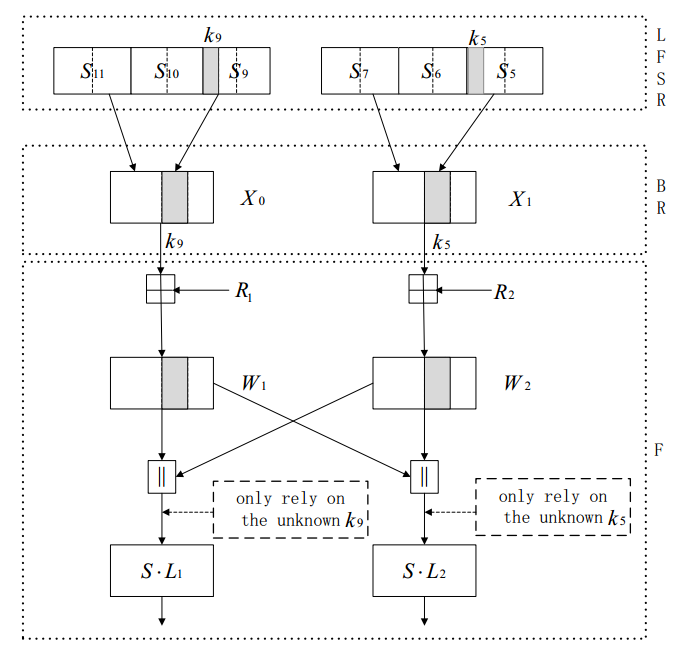
\includegraphics[height=.5\textheight]{../images/zuc_attack.png}
    \caption{非线性函数中左侧寄存器的输出仅和 k9 相关,右侧寄存器的输出仅和 k5 相关\cite{zuc_attack_tangming}}
    \label{fig:zuc_attack}
\end{figure}

我们来详细地讨论一下,是怎样得到这个中间值的



因此,选择初始化阶段第一轮打乱操作中,非线性函数右半部分的输出作为我们的中间值,尝试攻击出 k5 的值。

选择这个位置作为中间值有两个原因:

\begin{enumerate}
    \item \textbf{这个位置仅仅和单个密钥字节(k5)相关,和其他的密钥字节没有任何关系。}这意味着我们只需要猜测 $2^8=256$ 中情况,大大减少了工作量。如果选择某个其他的中间值,很可能和多个密钥字节有关联,我们假设关联的密钥字节数为 N,那么我们就需要猜测 $2^{8 \times N}$ 中情况。可以想象,如果关联的密钥字节很多的话,我们需要猜测的可能情况就会爆炸式增长,由于我们只拥有有限的计算资源,因此这是不能接受的。
    \item \textbf{这个位置是非线性变换(S 盒置换)的输出,因而正确猜测和错误猜测之间的差异较为明显。}这一点我们在上面已经提及,因此不再赘述。
\end{enumerate}

\vspace*{\baselineskip}

选择好了中间值,我们就可以通过编程计算出所有密钥猜测(从 0 到 255,也即 16 进制的 00 到 FF)对应的的中间值。

有了中间值之后,我们就可以根据汉明重量模型,计算出理论功耗值(也就是假设功耗值)。然后我们实施相关系数攻击,也即计算假设功耗值和实际功耗值之间的相关系数(在本次实验中,这个值还需要稍微处理一下,得到更加可靠的相对相关系数),然后分析相对相关系数,值最大的即对应最优的密钥猜测。

这就是对 ZUC 算法进行功耗分析攻击的大致流程,我们将在下一小节展示相关的实验结果,并补充一些实现细节。

\section{本章小结}




我们讨论了功耗分析中简单功耗分析和差分功耗分析的异同,并且重点介绍了差分功耗攻击的基本流程和一般方法。

最后我们讨论了针对 ZUC 算法的差分功耗分析方案,除了介绍了传统的差分功耗分析的流程,还依据相关资料选取了有效的中间值,并且解释了这样选取的具体原因。
